\documentclass{beamer}
\usepackage[utf8]{inputenc}
\usepackage[T1]{fontenc}
\usepackage[french]{babel}
\usepackage{colortbl}
\usepackage{verbatim}
  
\usetheme{Warsaw}

\title[Classification de documents]{Extraction de connaissances avancée\\ \emph{``Analyse d'opinion''}}
\author{Carbonnel Jessie \and Nguyen Daniel \and Pibre Lionel}
\institute[UM2]{Université de Montpellier 2}
\date{18 Décembre 2014}
\logo{
\includegraphics[height=10mm]{imgs/um2.png}}

\AtBeginSection[]
{
  \begin{frame}
  \frametitle{Sommaire}
  \tableofcontents[currentsection, hideothersubsections, hideothersections]
  \end{frame} 
}

\addtobeamertemplate{footline}{\insertframenumber/\inserttotalframenumber}

\setbeamertemplate{navigation symbols}{% 
}

\begin{document}

\begin{frame}
\titlepage
\end{frame}

\begin{frame}{Sommaire}
	\tableofcontents[hidesubsections]
\end{frame}
%%%%%%%%%%%%%%%%%
% SECTION
%%%%%%%%%%%%%%%%%
\section{Introduction}
\begin{frame}
	\begin{block}{Introduction}
		\textbf{Sujet:} Classification des opinions sur les commentaires des applications de Google Play Store.		
		
		\vspace{0.5cm}
		
		\textbf{Problématique:} Prédire la note que l'utilisateur va donner à une application à partir de son commentaire.
			
	\end{block}
\end{frame}

\section{Constitution du corpus}
\begin{frame}
	\begin{block}{Structure des données récupérées}
		\begin{verbatim}
			NomApplication:Ebook et PDF Reader
			IdApplication:books.ebook.pdf.reader
			CategorieApplication:Livres et références
			NoteApplication:4,3
			NombreVotants:43 379
			TitreCommentaire:Ebook Pelerin
			Commentaire: Super installation, ai acheté un ebook chez Bayard. Suis pas déçu.
			DateCommentaire:26 juillet 2014
			NoteCommentaire:5
		\end{verbatim}
	\end{block}
\end{frame}

\section{Prétraitement et génération des fichiers ARFF}
\subsection{Prétraitement}
\begin{frame}
	\begin{block}{TreeTagger}
		Utilisation de TreeTagger afin d'avoir la classe grammaticale des mots ainsi que leur forme lemmatisée.
	\end{block}
	
\end{frame}

\begin{frame}
\begin{exampleblock}{Structure de sortie de TreeTagger}
			\centering
			 \begin{tabular}{|c|c|c|}
					\hline
					Mot&Classe grammaticale&Mot lemmatisé\\
					\hline
					dès&PRP&dès\\
					que&KON&que\\
					je&PRO:PER&je\\
					lance&VER:pres&lancer\\
					l'&DET:ART&le\\
					application&NOM&application\\
					j'&PRO:PER&je\\
					adore&VER:pres&adorer\\
					cyprien&ADJ&cyprien\\
					\dots&\dots&\dots\\
					\hline
			 \end{tabular}
	\end{exampleblock}

\end{frame}

\subsection{Génération des fichiers ARFF}
\begin{frame}

\end{frame}

\section{Visualisation}
\subsection{Camembert}
\begin{frame}
	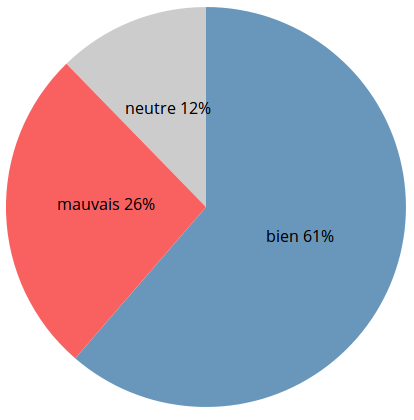
\includegraphics[height=5cm]{imgs/visu1.png}
\end{frame}

\subsection{Histogramme}
\begin{frame}
	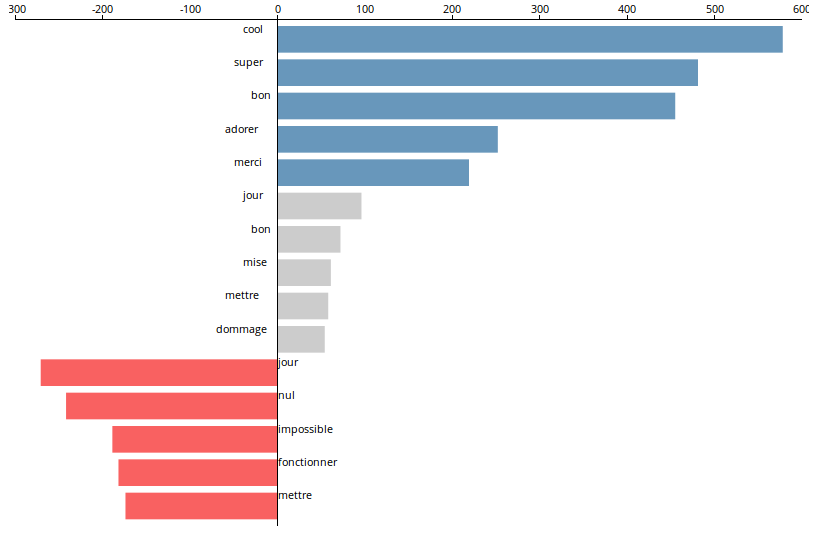
\includegraphics[height=5cm]{imgs/visu2.png}
\end{frame}

\section{Classification}
\begin{frame}
	\begin{block}{Algorithmes utilisés}
		\begin{itemize}
			\item NaiveBayes: probabiliste
			\item J48: arbre de décision
			\item JRip: règles d'association
			\item SMO: machine à vecteurs de support
			\item IBk: K plus proches voisins
		\end{itemize}
	\end{block}
\end{frame}

\begin{frame}
	\begin{block}{Les problèmes liés au corpus}
		\begin{itemize}
			\item Certains commentaires sont écrits en anglais
			\item Fautes d'orthographe et de frappe
		\end{itemize}
	\end{block}
\end{frame}

\begin{frame}
	\begin{exampleblock}{Fautes d'orthographe et de frappe}
		``Je kiff grave car jadore cyprien et jaimefai lui poser un question : est ce que tu connais squeezie ( ca c oui c sur ) norman kihouu tal blackm ....''\\
		
	%	
\includegraphics[height=20mm]{imgs/wtf.jpg}
	\end{exampleblock}
	
	\begin{exampleblock}{Commentaire en anglais}
		``It keeps loosing my books , I have to re-download them every day''
	\end{exampleblock}

\end{frame}

\begin{frame}
	\begin{block}{Résultats des instances correctments classifiées}
		\begin{description}
			\item[SMO: ]73,6\%
			\item[J48: ]69,3\%
			\item[NaiveBayes: ]67,8\%
			\item[JRip :]67,7\%
			\item[IBk :]64,4\%
		\end{description}	
	\end{block}
\end{frame}

\begin{frame}
	\begin{block}{Analyses des résultats}
		L'algorithme de classification SMO est le plus robuste.
		
		Les autres algorithmes sont plus sensibles au bruit et aux fautes d'orthographe.
	\end{block}
\end{frame}

\section{Conclusion et perspectives}
\begin{frame}

\end{frame}


\end{document}